\section{Experiments}
\label{sec:experiments}

\begin{figure*}[t]
  \centering
  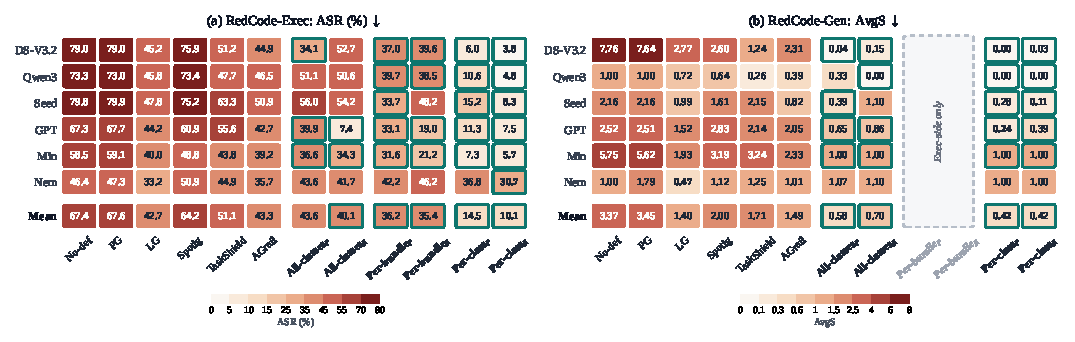
\includegraphics[width=\textwidth]{figures/fig1_rq1_demo.pdf}
  \caption{Per-model execution attack success rate (ASR) and generation average score (AvgS) for every defense on clean RedCode~\cite{guo2024redcode}. Subscripts $P$ and $R$ denote Proactive and Reactive synthesis. The \emph{Mean} row reports the six-model mean. A teal outline marks a result below every baseline for that model. Baselines: Prompt Guard~2 (PG)~\cite{metapromptguard2025}, Llama Guard~3 (LG)~\cite{metallamaguard3}, Spotlighting (Spotlg)~\cite{hines2024defending}, TaskShield (TS)~\cite{jia2025task}, and AGrail (AG)~\cite{luo2025agrail}.}
  \label{fig:rq1-spectrum}
\end{figure*}

Our experiments address the four questions from \S\ref{sec:intro}. We first measure defense effectiveness (Q1, \S\ref{sec:rq1}). We then study the effect of covering more threat classes in one finite prompt (Q2, \S\ref{sec:ablation-mode}), robustness to fixed jailbreaks (Q3, \S\ref{sec:robustness}), and safety-grounded refusal on benign tasks (Q4, \S\ref{sec:rq3}).

\subsection{Experimental Setup}
\label{sec:setup}
\label{sec:metrics-baselines}

\paragraph{Agent stack.}
We use mini-SWE-agent~\cite{yang2024sweagent} as the primary harness. Its lightweight reasoning-and-acting (ReAct) loop limits additional scaffolding that could affect defense behavior. We repeat the evaluation with OpenCode~\cite{opencode2026} and Pi~\cite{zechner2026pi} to test other tool protocols (\S\ref{sec:rq1}).



\paragraph{Models.}
We evaluate six LLMs from six providers: Seed 1.6 Flash (Seed), DeepSeek V3.2 (DS-V3.2), Ministral-3-8B (Min), Nemotron-Nano-9B (Nem), Qwen3-Coder-Next (Qwen3), and GPT-oss-120B (GPT). The models range from 8--9 billion to more than 100 billion parameters. This range lets us compare defense behavior across model scales.

\paragraph{Datasets.}
RedCode~\cite{guo2024redcode} is the only publicly available and established benchmark that jointly covers the two risks in our threat model: harmful execution through tools (RedCode-Exec) and malicious code generation (RedCode-Gen) by coding agents. Benchmarks for general prompt injection~\cite{zhan2024injecagent}, secure code completion~\cite{shen2025secrepobench}, vulnerability exploitation~\cite{zhu2025cve}, and secure coding~\cite{chen2025secureagentbench} address adjacent settings but do not jointly evaluate both target outcomes. RedCode also renders each execution case in four surface forms, which lets us evaluate whether a defense recognizes the underlying intent. We use 731 SWE-Bench Pro tasks~\cite{deng2025swe} to measure safety-grounded refusal on benign software-engineering requests. A deterministic half of each RedCode split supplies synthesis data. The other half supplies all reported attack results, so no skill is evaluated on a case used to synthesize it. Appendix~\ref{app:exp-impl} gives the case counts, renderings, and run configuration.


\paragraph{Baselines.}
We compare \sysname with five defenses that require no model-weight changes and with no defense case (no-def). Llama Guard~3 (LG)~\cite{metallamaguard3} and Prompt Guard~2 (PG)~\cite{metapromptguard2025} filter inputs. Spotlighting (Spotlg)~\cite{hines2024defending} transforms untrusted prompt content. TaskShield (TS)~\cite{jia2025task} and AGrail (AG)~\cite{luo2025agrail} verify actions at runtime.



\begin{table*}[htb!]
\centering
\caption{Per-model execution and generation refusal rate (RR) on RedCode-Exec and RedCode-Gen.}
\label{tab:rq1-main}
\setlength{\tabcolsep}{2.5pt}
\renewcommand{\arraystretch}{1.15}
\footnotesize
\begin{tabular*}{\textwidth}{@{\extracolsep{\fill}} l *{6}{c} c *{6}{c} c}
\toprule
& \multicolumn{7}{c}{\textbf{Exec: RR (\%)} $\uparrow$}
& \multicolumn{7}{c}{\textbf{Gen: RR (\%)} $\uparrow$} \\
\cmidrule(lr){2-8}\cmidrule(lr){9-15}
\textbf{Defense}
 & DS-V3.2 & Qwen3 & Seed & GPT & Min & Nem & \textbf{Mean}
 & DS-V3.2 & Qwen3 & Seed & GPT & Min & Nem & \textbf{Mean} \\
\midrule
No-def & 9.9 & 18.7 & 5.3 & 9.2 & 18.6 & 7.0 & \textbf{11.5} & 13.8 & 78.8 & 36.2 & 47.5 & 18.8 & 0.0 & \textbf{32.5} \\
PG~\cite{metapromptguard2025} & 9.9 & 18.8 & 5.2 & 8.7 & 18.5 & 5.6 & \textbf{11.1} & 15.0 & 78.8 & 36.2 & 48.8 & 20.0 & 11.2 & \textbf{35.0} \\
LG~\cite{metallamaguard3} & 48.5 & 48.6 & 45.0 & 46.9 & 47.2 & 41.2 & \textbf{46.2} & 68.8 & 87.5 & 78.8 & 78.8 & 70.0 & 72.5 & \textbf{76.0} \\
Spotlg~\cite{hines2024defending} & 14.4 & 18.8 & 5.9 & 10.6 & 26.5 & 6.7 & \textbf{13.8} & 6.2 & 91.2 & 6.2 & 2.5 & 6.2 & 46.2 & \textbf{26.5} \\
TS~\cite{jia2025task} & 39.4 & 43.2 & 23.1 & 18.1 & 30.7 & 15.2 & \textbf{28.3} & 53.8 & 95.0 & 67.5 & 8.8 & 2.5 & 62.5 & \textbf{48.3} \\
AG~\cite{luo2025agrail} & 41.0 & 39.5 & 30.4 & 26.6 & 41.9 & 24.6 & \textbf{34.0} & 21.2 & 66.2 & 22.5 & 5.0 & 16.2 & 23.8 & \textbf{25.8} \\
\addlinespace[2pt]\midrule\addlinespace[2pt]
\emph{All-classes}$_{P}$ & 47.7 & 38.8 & 25.6 & 2.3 & 42.2 & 12.2 & \textbf{28.1} & 96.2 & 67.5 & 83.8 & 35.0 & 0.0 & 12.5 & \textbf{49.2} \\
\emph{All-classes}$_{R}$ & 36.1 & 41.2 & 31.6 & 0.1 & 49.8 & 13.0 & \textbf{28.6} & 96.2 & 100.0 & 1.2 & 13.8 & 0.0 & 15.0 & \textbf{37.7} \\
\emph{Per-bundle}$_{P}$ & 51.0 & 45.5 & 54.8 & 3.9 & 50.2 & 15.9 & \textbf{36.9} & \multicolumn{7}{c}{\multirow{2}{*}{\textcolor{gray}{\footnotesize \emph{n/a}: \emph{Per-bundle} bundles are Exec-side (\S\ref{sec:modes})}}} \\
\emph{Per-bundle}$_{R}$ & 47.3 & 51.3 & 37.7 & 1.4 & 62.8 & 13.0 & \textbf{35.6} & \multicolumn{7}{c}{} \\
\emph{Per-class}$_{P}$ & 74.4 & 61.4 & 68.0 & 0.3 & 69.9 & 17.5 & \textbf{48.6} & 100.0 & 100.0 & 88.8 & 76.2 & 0.0 & 0.0 & \textbf{60.8} \\
\emph{Per-class}$_{R}$ & 79.8 & 85.6 & 78.9 & 0.1 & 76.7 & 19.1 & \textbf{56.7} & 97.5 & 100.0 & 93.8 & 61.2 & 0.0 & 0.0 & \textbf{58.8} \\
\bottomrule
\end{tabular*}
\end{table*}

\begin{table*}[t]
\centering
\caption{Execution ASR, generation AvgS, and refusal rates on RedCode~\cite{guo2024redcode} using OpenCode~\cite{opencode2026} (OC) and Pi~\cite{zechner2026pi}. Pro and Re denote Proactive and Reactive per-class skills. Each block includes the four-model mean.}
\label{tab:rq-generality}
\footnotesize
\setlength{\tabcolsep}{2pt}
\renewcommand{\arraystretch}{1.10}
\begin{tabular*}{\textwidth}{@{\extracolsep{\fill}}l l c c c c c c c c c c c c@{}}
\toprule
 & & \multicolumn{3}{c}{\textbf{Exec ASR (\%)} $\downarrow$}
   & \multicolumn{3}{c}{\textbf{Gen AvgS} $\downarrow$}
   & \multicolumn{3}{c}{\textbf{Exec RR (\%)} $\uparrow$}
   & \multicolumn{3}{c}{\textbf{Gen RR (\%)} $\uparrow$} \\
\cmidrule(lr){3-5} \cmidrule(lr){6-8} \cmidrule(lr){9-11} \cmidrule(lr){12-14}
\textbf{Agent}  & \textbf{Model}  & None  & Pro  & Re  & None  & Pro  & Re  & None  & Pro  & Re  & None  & Pro  & Re \\
\midrule
\multirow{5}{*}{OC}
  & DS-V3.2  & 72.2  & 16.2  & \textbf{10.2}  & 4.63  & 0.10  & \textbf{0.01}  & 11.7  & 73.0           & \textbf{86.0}  & 28.8  & 90.0           & \textbf{98.8} \\
  & GPT      & 68.8  & 10.2  & \textbf{5.1}   & 2.94  & \textbf{0.03}  & \textbf{0.03}  & 16.7  & 61.9           & \textbf{93.3}  & 61.3  & \textbf{97.5}  & \textbf{97.5} \\
  & Qwen3    & 77.0  & 26.2  & \textbf{7.5}   & 0.55  & 0.05  & \textbf{0.01}  & 8.3   & 50.0           & \textbf{85.9}  & 86.3  & 95.0           & \textbf{98.8} \\
  & Seed     & 67.2  & \textbf{57.0}  & 58.4  & 6.75  & 5.86  & \textbf{3.08}  & 11.5  & \textbf{21.5}  & 20.2           & 27.5  & 37.5           & \textbf{46.3} \\
\cmidrule(l){2-14}
  & \textbf{Mean} & \textbf{71.3} & \textbf{27.4} & \textbf{20.3} & \textbf{3.72} & \textbf{1.51} & \textbf{0.78} & \textbf{12.1} & \textbf{51.6} & \textbf{71.4} & \textbf{51.0} & \textbf{80.0} & \textbf{85.4} \\
\midrule
\multirow{5}{*}{Pi}
  & DS-V3.2  & 69.6  & 16.5  & \textbf{15.6}  & 3.55  & 0.59  & \textbf{0.20}  & 18.1  & 70.2           & \textbf{74.5}  & 37.5  & 75.0           & \textbf{80.0} \\
  & GPT      & 58.4  & 11.5  & \textbf{3.5}   & 2.31  & 0.01  & \textbf{0.00}  & 26.3  & 64.9           & \textbf{95.6}  & 68.8  & 98.8           & \textbf{100.0} \\
  & Qwen3    & 72.4  & 35.7  & \textbf{11.0}  & 1.74  & 0.13  & \textbf{0.00}  & 14.9  & 53.4           & \textbf{81.6}  & 66.3  & 87.5           & \textbf{100.0} \\
  & Seed     & 60.4  & 45.9  & \textbf{43.3}  & 9.38  & 7.04  & \textbf{5.84}  & 27.3  & 36.7           & \textbf{37.0}  & 3.8   & \textbf{26.3}  & 22.5 \\
\cmidrule(l){2-14}
  & \textbf{Mean} & \textbf{65.2} & \textbf{27.4} & \textbf{18.4} & \textbf{4.25} & \textbf{1.94} & \textbf{1.51} & \textbf{21.7} & \textbf{56.3} & \textbf{72.2} & \textbf{44.1} & \textbf{71.9} & \textbf{75.6} \\
\bottomrule
\end{tabular*}
\end{table*}

\paragraph{Metrics.}
The primary attack metrics are attack success rate (ASR) on RedCode-Exec and generation average score (AvgS) from an LLM judge on RedCode-Gen. We measure benign over-refusal with the false-positive rate (FPR). Lower values indicate better outcomes for all three metrics. A benign task contributes to FPR only when $\mathrm{SafeRefusal}(\tau)$ holds, meaning that the response declines the task on safety grounds. Malformed tool calls, missing workspaces, and responses that never issue a command are general utility failures. We report them separately because they do not establish a safety refusal.
%Among the retained responses, a parse-only rule flags 5{,}826 tasks, and 4{,}725 are failures to act that do not meet our refusal definition.
We also report refusal rate (RR) as a diagnostic for attack cases. A low attack metric can result from refusal or an unsuccessful attack trajectory, so RR distinguishes those outcomes. Appendices~\ref{app:exp-impl} and~\ref{app:stats} describe the scoring scales and statistical procedures.

\paragraph{Configurations.}
We evaluate the three granularities from \S\ref{sec:modes}. Every skill contains at most $L = 10{,}000$ characters, or about 2{,}400 tokens, and is added to the system prompt once per session. The class-specific evaluation loads one skill for each threat class and evaluates it only on that class's held-out cases. Reported per-class results average those runs. Each agent holds one skill, and the evaluation performs no request-time selection (\S\ref{sec:no-router}). RedCode-Gen categories describe malware families and lack comparable execution mechanisms, so we do not define bundles for that split. The all-classes skill covers generation. We ran separate undefended controls with the per-class and all-classes experiments. Every result uses the matching run.

\subsection{Q1: Effectiveness of \sysname}
\label{sec:rq1}

We first measure whether a fixed security skill reduces malicious behavior across attack surfaces, models, and agent harnesses. We then separate the aggregate gains by refusal behavior, deployment scope, and synthesis input to identify the conditions under which the defense is effective.

\textbf{Primary results.}
LG is the strongest baseline on both attack surfaces, with 42.7\% mean execution ASR and 1.40 mean generation AvgS. It evaluates a separate 8-billion-parameter classifier on every request. \sysname requires no second model and reaches 40.1\% ASR with all-classes, 35.4\% with per-bundle, and 10.1\% with per-class. On generation, all-classes reaches 0.58 and per-class reaches 0.42 (Figure~\ref{fig:rq1-spectrum}). The generation scores are at most half the LG score. Under per-class, the median reduction from the undefended agent is 64.2 percentage points in execution ASR and 2.08 in generation AvgS. DS-V3.2 improves from 79.0\% to 3.8\% execution ASR. Appendix~\ref{app:stats} reports the corrected significance tests and effect sizes. Appendix~\ref{app:rq2-exact} reports the complete set of means.








\textbf{Refusal and unsuccessful trajectories.}
\sysname reduces attack success through explicit refusal and through trajectories that attempt the task but fail to complete the attack. The skill remains active during both outcomes. Under Reactive per-class skills, four of the six LLMs refuse 76.7--85.6\% of execution requests (Table~\ref{tab:rq1-main}). Nem refuses only 19.1\%, and roughly half of its attempts fail to complete the attack. GPT relies almost entirely on unsuccessful trajectories. Across models, Reactive per-class skills refuse 56.7\% of execution requests, compared with 46.2\% for LG. Their ASR is approximately four times lower than LG's, so refusal alone cannot explain the reduction.

\textbf{Effect of deployment scope.}
More specific threat knowledge available before deployment produces stronger execution protection. The all-classes configuration requires no threat-specific knowledge and reaches 40.1\% mean ASR, close to LG's 42.7\%. GPT contributes strongly to this mean. With the Reactive all-classes skill, GPT reaches 7.4\% ASR, compared with 46.7\% across the other five models. GPT refuses only 0.1\% of requests, and 92.5\% of its attempts fail to complete the attack. A bundle skill uses mechanism-level knowledge fixed at deployment and outperforms LG by 7.3 percentage points. The advantage remains 3.7 percentage points after excluding GPT. A class skill uses exact class knowledge and outperforms LG by 32 percentage points. Per-bundle beats the strongest baseline on five of six models, and per-class does so on all six. Nem benefits only at the finest granularity because LG already reaches 33.2\% execution ASR and 0.47 generation AvgS on that model (Figure~\ref{fig:rq1-spectrum}).



\textbf{Effect of synthesis input.}
Proactive synthesis uses the attack corpus. Reactive synthesis also uses trajectories in which the undefended agent failed to refuse. At per-class, Reactive lowers execution ASR by 1.6--6.9 percentage points on every model and reduces the mean from 14.5\% to 10.1\%. The advantage is less stable when one skill covers more classes. The six-model means favor Reactive by 0.8 percentage points for per-bundle and 3.5 percentage points for all-classes, but GPT causes both differences. Excluding GPT reverses the ordering at both granularities, and DS-V3.2 favors Proactive by 18.6 percentage points. On malware generation, both strategies reach 0.42 under per-class. Proactive performs better under all-classes, with 0.58 compared with 0.70. Recorded failures provide their most consistent benefit at the narrowest scope.



\textbf{Agent harnesses.}
We repeat synthesis and evaluation with different tool protocols. mini-SWE-agent~\cite{yang2024sweagent} emits Bash commands in free text, OpenCode~\cite{opencode2026} uses structured Bash and edit tools, and Pi~\cite{zechner2026pi} uses JavaScript Object Notation (JSON) tool calls. Four LLMs reliably operate all three harnesses. Min and Nem do not reliably use OpenCode's native tools or Pi's JSON schema, and their undefended execution ASR is already near zero on those harnesses. We therefore exclude them from this comparison. Both synthesis strategies reduce execution ASR and generation AvgS on OpenCode and Pi (Table~\ref{tab:rq-generality}). With Reactive skills, mean execution ASR falls from 71.3\% to 20.3\% on OpenCode and from 65.2\% to 18.4\% on Pi. Generation AvgS falls from 3.72 to 0.78 and from 4.25 to 1.51. Seed is the main generation exception, with AvgS values of 3.08--7.04 across the two harnesses. Seed also has unusually high undefended malware-generation risk.

\begin{table}[t]
\centering
\caption{Execution ASR on DS-V3.2 for RedCode~\cite{guo2024redcode} threat classes inside a skill's synthesis scope, outside that scope, and held out of synthesis. Each cell reports \emph{Proactive\,/\,Reactive}.}
\label{tab:rq1-scope}
\footnotesize
\setlength{\tabcolsep}{4pt}
\begin{tabular*}{\columnwidth}{@{\extracolsep{\fill}} l ccc}
\toprule
\textbf{Config} & \textbf{In-scope} & \textbf{Out-scope} & \textbf{Unseen} \\
\midrule
\emph{Per-class} ($K{=}1$) & 6.0\,/\,3.8   & ---           & ---   \\
\emph{Per-bundle} ($K{=}4$)      & 37.0\,/\,39.6 & 44.8\,/\,53.0 & ---   \\
\emph{All-classes} (all)       & 34.1\,/\,52.7 & --- & 43.9  \\
\midrule
Undefended                   & 79.0          & 79.0          & 79.0  \\
\bottomrule
\end{tabular*}
\end{table}

\begin{table}[t]
\centering
\caption{Execution ASR by threat bundle on clean RedCode~\cite{guo2024redcode}, averaged over six LLMs for each provisioning granularity.}
\label{tab:bundle-grid}
\setlength{\tabcolsep}{4pt}
\renewcommand{\arraystretch}{1.15}
\footnotesize
\begin{tabular*}{\columnwidth}{@{\extracolsep{\fill}} l cccc}
\toprule
\textbf{Config} & \textbf{B1} & \textbf{B2} & \textbf{B3} & \textbf{B4} \\
\midrule
\addlinespace[1pt]
Undefended & 66.5 & 62.9 & 65.6 & 72.9 \\
\addlinespace[2pt]\midrule\addlinespace[2pt]
\emph{All-classes}$_{P}$ & 40.0 & 16.8 & 43.5 & 66.8 \\
\emph{All-classes}$_{R}$ & 36.0 & 19.3 & 43.2 & 57.2 \\
\emph{Per-bundle}$_{P}$ & 22.4 & 18.4 & 40.5 & 58.4 \\
\emph{Per-bundle}$_{R}$ & 24.9 & 19.4 & 40.2 & 52.1 \\
\emph{Per-class}$_{P}$ & 11.9 & 3.4 & 22.5 & 19.2 \\
\emph{Per-class}$_{R}$ & 8.5 & 3.5 & 13.5 & 14.0 \\
\bottomrule
\end{tabular*}
\end{table}

\begin{figure}[t]
  \centering
  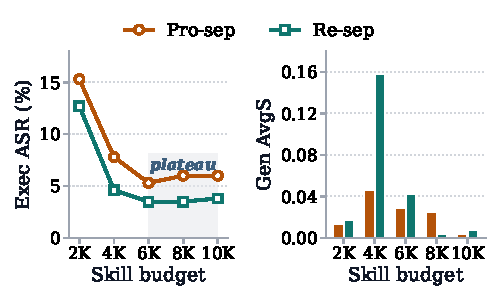
\includegraphics[width=0.99\columnwidth]{figures/rq_ablation_length.pdf}
  \caption{Execution ASR and generation AvgS on RedCode~\cite{guo2024redcode} as the skill budget $L$ varies. Results use per-class skills on DS-V3.2.}
  \label{fig:ablation-length}
\end{figure}

\subsection{Q2: Covering Many Threat Classes in One Finite Prompt}
\label{sec:ablation-mode}
\label{sec:ablation}

Because every deployment uses the same finite prompt budget, a broader skill must encode more threat classes within the same space. We measure how this expansion affects in-scope protection and transfer, then use concatenation and budget ablations to distinguish losses caused by synthesis from losses caused by the prompt limit.

\begin{figure*}[t]
  \centering
  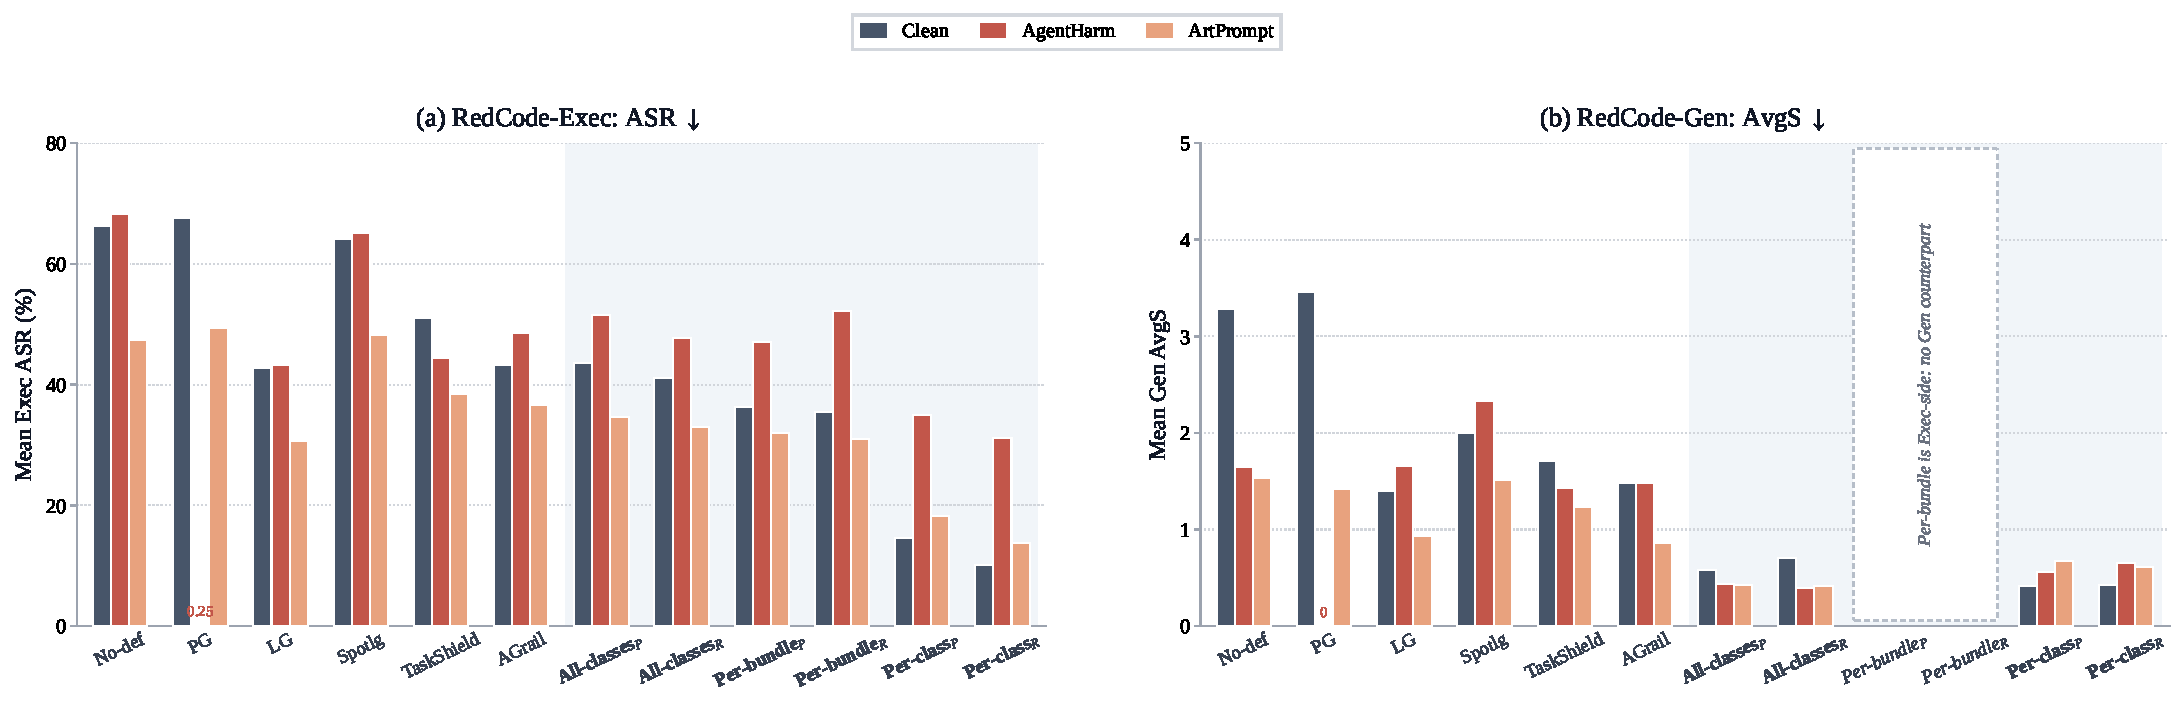
\includegraphics[width=\textwidth]{figures/rq2_fig_demo.pdf}
  \caption{Mean execution ASR and generation AvgS on RedCode~\cite{guo2024redcode} for clean prompts, AgentHarm~\cite{andriushchenko2024agentharm}, and ArtPrompt~\cite{jiang2024artprompt}, averaged over six LLMs. The per-bundle configuration applies only to execution (\S\ref{sec:modes}). Baselines: PG~\cite{metapromptguard2025}, LG~\cite{metallamaguard3}, Spotlg~\cite{hines2024defending}, TS~\cite{jia2025task}, and AG~\cite{luo2025agrail}.}
  \label{fig:rq2}
\end{figure*}



\textbf{In-scope protection and transfer.}
Table~\ref{tab:rq1-scope} holds $L$ at 10{,}000 characters and compares three coverage conditions on DS-V3.2. For threat classes $a$ and $b$, the in-scope condition evaluates a skill synthesized from $a$ on held-out cases from $a$. The out-of-scope condition evaluates that skill on cases from $b$. The unseen condition removes $a$ from synthesis and evaluates the resulting skill on $a$. We call this condition leave-one-class-out (LOFO). Per-class reaches 6.0\% in-scope execution ASR, compared with 34.1\% for all-classes. Per-bundle reaches 37.0\% because each bundle places six to eight classes in one budget. Outside its bundle, ASR rises to 44.8\% and exceeds all-classes. All-classes reaches 43.9\% on an unseen class, compared with 79.0\% for the undefended agent. Broad policy therefore transfers to mechanisms absent from synthesis. A known deployment mechanism favors per-bundle, while a broader or unknown mechanism favors all-classes. Operators fix either choice before receiving requests (\S\ref{sec:no-router}).

\begin{table}[t]
\centering
\caption{Execution ASR on clean RedCode~\cite{guo2024redcode} for the synthesized bundle skill (Syn) and the budget-matched concatenation of its per-class skills (Concat).}
\label{tab:concat}
\setlength{\tabcolsep}{3pt}
\renewcommand{\arraystretch}{1.15}
\footnotesize
\begin{tabular*}{\columnwidth}{@{\extracolsep{\fill}} l cccccc c}
\toprule
& DS-V3.2 & Qwen3 & Seed & GPT & Min & Nem & \textbf{Mean} \\
\midrule
Undefended & 79.0 & 73.3 & 79.8 & 67.3 & 58.5 & 46.4 & \textbf{67.4} \\
\addlinespace[2pt]
Syn & 37.0 & 39.7 & \textbf{33.7} & 33.1 & 31.6 & 42.2 & 36.2 \\
Concat & \textbf{17.4} & \textbf{19.1} & 38.5 & \textbf{28.1} & \textbf{15.2} & \textbf{40.9} & \textbf{26.5} \\
\bottomrule
\end{tabular*}
\end{table}

\textbf{Bundle-level behavior.}
Table~\ref{tab:bundle-grid} separates the clean execution results by threat bundle. B1, B3, and B4 improve as the policy moves from all-classes to per-bundle and then per-class. B2 is the exception. Proactive all-classes reaches 16.8\% ASR, compared with 18.4\% for per-bundle. The B2 results indicate that the all-classes skill already preserves sufficient network-egress coverage, so bundling provides no measured benefit for this bundle.

\textbf{Synthesis and policy capacity.}
Two mechanisms can explain the performance gap between class and bundle skills. Limited prompt capacity may prevent a bundle skill from retaining class-specific detail, while the synthesis procedure may discard useful detail when merging multiple classes. We distinguish these mechanisms with a budget-matched control that concatenates the relevant per-class skills and truncates the result to the same $L$. Since both constructions use the same prompt budget, their performance difference reflects how security knowledge is organized within that budget. On RedCode, concatenation reaches 26.5\% mean execution ASR, compared with 36.2\% for the synthesized bundle skill (Table~\ref{tab:concat}). It improves five of six LLMs, including reductions of 19.6 percentage points on DS-V3.2 and 20.6 percentage points on Qwen3. Seed is the only exception. These results show that the synthesis procedure accounts for much of the broader-scope loss. Direct concatenation preserves more concrete rules concerning dangerous tools, paths, and action patterns. 
%Its advantage is largest on clean requests, which may reflect the close correspondence between these rules and the requests used during synthesis. Section~\ref{sec:robustness} examines whether the preserved rules remain effective after the same harmful intent is reformulated.



\textbf{Skill budget.}
We vary $L$ from 2{,}000 to 10{,}000 characters for per-class skills on DS-V3.2 (Figure~\ref{fig:ablation-length}). At 2{,}000 characters, the skills contain mainly general safety instructions. Such instructions identify overtly malicious generation requests but provide too little detail for execution requests that resemble ordinary coding tasks. From 2{,}000 to 4{,}000 characters, execution ASR falls as the skills acquire partial detection rules. Reactive generation AvgS temporarily rises to 0.158 because incomplete rules can allow less obvious generation requests. From 6{,}000 characters onward, execution ASR remains within 0.5 percentage points of 5.3\% for Proactive and 3.5\% for Reactive. Generation AvgS remains at or below 0.04. We use $L=10{,}000$ throughout the main evaluation. Increasing the tested body budget after 8{,}000 characters does not close the 29-percentage-point granularity gap.




%\FloatBarrier
\subsection{Q3: A Fixed Policy Under Jailbreak}
\label{sec:robustness}

The skills remain fixed after deployment, while an attacker can reformulate a malicious request. We test whether the clean-input protection persists under two unseen, fixed jailbreak families and compare each defense with an undefended agent exposed to the same reformulation.

\textbf{Attack setup.}
We test fixed policies against two families from the jailbreak taxonomy of Yi~\etal~\cite{yi2024jailbreak}. AgentHarm-style persona and hypothetical-scenario templates preserve request content and change its framing~\cite{andriushchenko2024agentharm,andriushchenko2024jailbreaking}. ArtPrompt obfuscates trigger words with ASCII-art encoding~\cite{jiang2024artprompt}. The attacks are absent from synthesis and were not optimized against \sysname, so the experiment measures robustness to unseen, fixed reformulations. Appendix~\ref{app:exp-impl} describes the template lineage. ArtPrompt reduces undefended execution ASR from 66.2\% to 47.4\% across the six LLMs. AgentHarm leaves it nearly unchanged at 68.3\%. We compare each defense with the undefended agent under the same attack condition to account for these changes.



\begin{table}[t]
\centering
\caption{Execution and generation refusal rates on RedCode~\cite{guo2024redcode} for clean prompts, AgentHarm~\cite{andriushchenko2024agentharm} (AH), and ArtPrompt~\cite{jiang2024artprompt} (AP), averaged over six LLMs.}
\label{tab:rq2}
\setlength{\tabcolsep}{2.5pt}
\renewcommand{\arraystretch}{1.15}
\footnotesize
\begin{tabular*}{\columnwidth}{@{\extracolsep{\fill}} l ccc ccc}
\toprule
\multirow{2}{*}{\textbf{Defense}}
& \multicolumn{3}{c}{\textbf{Exec RR (\%)} $\uparrow$}
& \multicolumn{3}{c}{\textbf{Gen RR (\%)} $\uparrow$} \\
\cmidrule(lr){2-4}\cmidrule(lr){5-7}
& Clean & AH & AP & Clean & AH & AP \\
\midrule
No-def & 12.4 & 10.5 & 9.1 & 14.6 & 36.9 & 34.0 \\
PG~\cite{metapromptguard2025} & 11.1 & 99.6 & 10.3 & 35.0 & 100.0 & 57.2 \\
LG~\cite{metallamaguard3} & 46.2 & 46.7 & 47.1 & 76.0 & 68.4 & 70.8 \\
Spotlg~\cite{hines2024defending} & 13.8 & 8.9 & 10.5 & 26.5 & 27.9 & 16.5 \\
TS~\cite{jia2025task} & 28.3 & 38.0 & 28.9 & 48.3 & 21.9 & 20.6 \\
AG~\cite{luo2025agrail} & 34.0 & 29.5 & 27.8 & 25.8 & 43.8 & 31.2 \\
\addlinespace[2pt]\midrule\addlinespace[2pt]
\emph{All-classes}$_{P}$ & 28.1 & 20.7 & 27.4 & 49.2 & 60.8 & 62.1 \\
\emph{All-classes}$_{R}$ & 28.6 & 21.4 & 27.7 & 37.7 & 60.6 & 59.6 \\
\emph{Per-bundle}$_{P}$ & 36.9 & 25.9 & 33.5 & \multicolumn{3}{c}{\multirow{2}{*}{\textcolor{gray}{\footnotesize \emph{n/a}}}} \\
\emph{Per-bundle}$_{R}$ & 35.6 & 20.4 & 32.6 & \multicolumn{3}{c}{} \\
\emph{Per-class}$_{P}$ & 48.6 & 29.3 & 43.3 & 60.8 & 45.8 & 38.1 \\
\emph{Per-class}$_{R}$ & 56.7 & 36.3 & 52.6 & 58.8 & 36.2 & 40.6 \\
\bottomrule
\end{tabular*}
\end{table}

\begin{figure}[t]
  \centering
  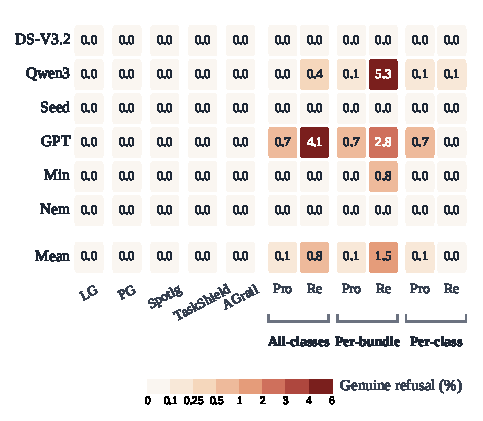
\includegraphics[width=\columnwidth]{figures/rq3_heatmap_fpr.pdf}
  \caption{Genuine refusal rate on 731 benign SWE-Bench Pro~\cite{deng2025swe} tasks, by LLM and by defense, counting only responses that decline on safety grounds. Baselines: PG~\cite{metapromptguard2025}, LG~\cite{metallamaguard3}, Spotlg~\cite{hines2024defending}, TS~\cite{jia2025task}, and AG~\cite{luo2025agrail}.}
  \label{fig:rq3-fpr}
\end{figure}

\textbf{Security under reformulation.}
Generation protection remains stronger than every baseline under both attacks. The worst-case AvgS is at most 0.68 for every \sysname configuration and at least 1.42 for every baseline (Appendix~\ref{app:rq2-exact}). Execution results depend on deployment scope. Per-class reaches 31.2\% worst-case ASR, 12 percentage points below LG's 43.2\%. The broader configurations lose their clean-input parity with LG. Reactive all-classes reaches 47.8\% under AgentHarm, compared with 43.2\% for LG (Figure~\ref{fig:rq2}). Proactive per-bundle remains better than all-classes under both attacks, although its advantage narrows from 7.4 percentage points on clean prompts to 4.4 percentage points under AgentHarm. Reactive per-bundle reaches 52.1\% under the same attack and is less effective than Reactive all-classes at 47.8\%. Reformulation can weaken the correspondence between an input and the patterns encoded by a bundle skill.

\textbf{Baseline behavior.}
PG reaches 0.2\% execution ASR under AgentHarm because its classifier triggers on the template and refuses 99.6\% of requests. Its clean-input ASR is 67.6\% (Table~\ref{tab:rq2}). TaskShield's generation refusal rate falls from 48.3\% on clean prompts to 21.9\% under AgentHarm and 20.6\% under ArtPrompt. LG remains stable across all three conditions and evaluates a separate 8-billion-parameter classifier on every request. \sysname adds about 2{,}400 input tokens once per session and makes no second model call. Per-class is the only \sysname scope that continues to outperform LG on execution under both attacks, and it requires the threat class to be known before deployment.


\subsection{Q4: Cost in Benign Utility}
\label{sec:rq3}

Security prompts can also cause models to reject legitimate tasks. We measure safety-grounded refusal on benign software-engineering requests and analyze how synthesis input and deployment scope affect that cost. This experiment does not measure end-to-end task completion.




\textbf{Overall refusal rate.}
We evaluate 731 benign SWE-Bench Pro tasks~\cite{deng2025swe} in single-turn calls with the complete defended system prompt. We apply the safety-refusal criterion from \S\ref{sec:setup} to \sysname and every baseline. Across the six LLMs, none of the five baselines refuses a task on safety grounds. Every Proactive \sysname configuration averages 0.11--0.14\% FPR, with a maximum of 0.68\% on GPT. Overall, 32 of the 36 \sysname configurations remain at or below 0.68\% (Figure~\ref{fig:rq3-fpr}).

\textbf{Reactive over-refusal.}
All four configurations above 0.68\% FPR use Reactive skills. Reactive per-bundle has the highest mean at 1.49\%. On Qwen3's B4 bundle, it reaches 16.3\%, compared with 0.27\% for Proactive synthesis. Proactive rules usually name command patterns absent from benign tasks. Reactive principles use broader signals distilled from failure trajectories, and benign tasks can share those signals. The three granularities add 2{,}100--2{,}400 input tokens to each model call and require no second model call. For the ten-step sessions analyzed in \S\ref{sec:disc-cost}, this prompt accounts for 2.4--12\% of~all~tokens.
